%%%%%%%%%%%%%%%%%%%%%%%%%%%%%%%%%%%%%%%%%%%%%%
\logvartrue
\chapter{The quest for the super-rhizobium}
%%%%%%%%%%%%%%%%%%%%%%%%%%%%%%%%%%%%%%%%%%%%%%

\section{Comparative genomics of \textit{S. meliloti}}
As shown in chapter \ref{chap:alpha}, inside the class Alphaproteobacteria there is a common genetic "toolbox" for the establishment of plant symbiosis; however, little is known about the intraspecific variability of the genes related to symbiosis and its relationships to the observed phenotypic variability, especially in the plant growth promotion phenotype. Up to date, only one strain of the nitrogen-fixing bacterium \textit{Sinorhizobium meliloti} was available \cite{galibert2001composite}, with a limited possibility to perform comparative genomics studies, even though experimental approaches like the Comparative Genomics Hybridization arrays (CGH) have been performed on four natural strains of \textit{S. meliloti}; about 5\% of the genes of this genome was found to be variable in the natural isolates of this species and the megaplasmid pSymA was found to be the hotspot for intra-specific differentiation, with the variable regions mainly grouped as clusters \cite{giuntini2005large}. The peculiar genomic composition of the \textit{S. meliloti} species, having three replicons, is also an interesting feature to be studied through comparative genomics, to understand if there is also a variability in the size of these replicons, on functional content and on their structure; thanks to the recent advances in sequencing technologies, the complete or draft genomic sequences of other natural isolates of this species have been sequenced: their genomic features with regard to plant symbiosis, nitrogen fixation and genome evolution are discussed in this chapter.

\newpage
\section{Exploring the symbiotic pangenome of the nitrogen fixing bacterium \textit{Sinorhizobium meliloti}}
The first comparative genomics analysis on the \textit{Sinorhizobium meliloti} species has been performed on the reference laboratory strain Rm1021 and two natural isolates: one from the Aral sea region, in Kazakhstan (strain AK83) and one from an agricultural field from Lodi, Italy (BL225C); their 
variability in the symbiotic phenotype has been already established \cite{biondi2009metabolic}. The presence of such an high variability should then be reflected in a different pattern of presence/absence of genes related to symbiosis, some of which may have been not yet characterized; regulatory features may also be related to the different observed phenotypes, as shown in a comparative genomics study of the cell cycle in \textit{Alphaproteobacteria} \cite{brilli2010diversity}.

\newpage
\includepdf[pages=-,offset=10mm 0, scale=0.9]{articles/Galardini2011.pdf}

\newpage
\section{Replicon-dependent bacterial genome evolution: the case of \textit{Sinorhizobium meliloti}}
Many bacterial species, such as the alphaproteobacterium \textit{Sinorhizobium meliloti}, are characterized by open pangenomes and strains contain multipartite genomes consisting of a chromosome and other large-sized replicons, such as chromids, megaplasmids and plasmids.
The evolutionary forces that shape the pangenome of species with multipartite genomes in both functional and structural aspects are still poorly understood. To shed light on this topic, we sequenced the genomes of ten \textit{S. meliloti} strains, which were combined in our analysis to four publicly-available additional genomic sequences.
Results obtained indicated that the three main replicons present in these strains (a chromosome, a chromid and a megaplasmid) show a partly independent history during strains differentiation. In particular, the chromid was shown to be a hotspot for positively-selected genes and, unexpectedly, genes resident in the chromid were also found to be more widespread in distant taxa than those located in the other replicons. Moreover, through the exploitation of a DNA proximity network, a series of conserved “DNA backbones” were found to shape the structural evolution of the genome, with the rest of the genome experiencing rearrangements. 
The presented data allow to depict a scenario where the evolution of the \textit{S. meliloti} pangenome includes a structurally-conserved genome fraction that evolves by positive selection (mainly on the chromid), and a highly-variable fraction, that mostly contributes to structural fluidity and to the emergence of new functions (the megaplasmid), then suggesting that the chromids could have had a distinctive role in intra-species differentiation\footnote{Authors: \textbf{Marco Galardini}, Francesco Pini, Marco Bazzicalupo, Emanuele G. Biondi, Alessio Mengoni}.

\subsection{Introduction}
The relative contribution of the forces that drive the evolution of organisms and genomes and the coupling between genome and phenome evolution have focused the attention of several investigators and lead to the formulation of new hypotheses on adaptive traits \cite{hughes2011evolution} and to the identification of possible rules governing the evolutionary process at large phylogenetic scale \cite{koonin2010constraints}. Concerning the evolutionary processes at the intra-species scale (\textit{microevolution}), prokaryotic organisms follow distinct patterns with respect to eukaryotic organisms. In particular, it is well known that, even in the same species, bacterial genomes of different strains often present a core and a dispensable genome, the core genome being common to all strains, while the dispensable genome comprises genes present only in one (unique) or in a subset of strains (accessory) \cite{tettelin2008comparative}. The dispensable genome, which can account for a large fraction of the entire pangenome, has been shown to harbor gene related to local adaptation functions, originated by relatively recent horizontal gene transfer events \cite{medini2008microbiology} and it may explain phenotypic differences found in natural strains \cite{biondi2009metabolic}; by looking at the proportion of the dispensable fraction over the core genome, it is also possible to speculate about the life-style of a given species \cite{tettelin2008comparative}. Moreover, concerning genome structure, several species contain multipartite genomes, that are genomes composed by several replicons; often the additional replicons show a size as large as the chromosome. Such additional large replicons are collectively called megaplasmids, but recently a new term “chromid” has been proposed to better describe the biological features of several megaplasmids, which present housekeeping functions (so they are chromosome-like) and plasmid replication and partition systems \cite{harrison2010introducing}; chromids have been claimed as signatures for genera evolution, while megaplasmids could be more species-specific elements. However, it is still unclear if chromosome, chromids and megaplasmids may follow commons or distinct evolutionary patterns at the intra-specific level. 
\textit{Sinorhizobium meliloti} is one of the most investigated model bacterial species for symbiotic interaction with plants \cite{gibson2008molecular}; it is found in different habitats, since it behaves as free-living bacterium in most of temperate soils, as symbiont in the root nodules of host leguminous plants, mainly of genera \textit{Medicago}, \textit{Melilotus} and \textit{Trigonella} (\textit{Fabaceae}) \cite{sprent2001nodulation}, and also as endophyte in host \cite{pini2012exploring} or non-host plant species \cite{chi2005ascending}. As model in evolutionary genomics \textit{S. meliloti} is particularly attracting since strains of this species harbor large and typically multipartite genomes with a chromosome, a chromid, a megaplasmid, plus additional smaller plasmids \cite{krawiec1990organization}\cite{galibert2001composite}\cite{galardini2011exploring}\cite{tian2012comparative}. Previous population genetics investigations have shown that strains of \textit{S. meliloti} are highly variable and various studies explored the relationship between the pattern of genetic variation and environmental variables, notably geographical separation and symbiotic preferences \cite{paffetti1996genetic} \cite{paffetti1998influence} \cite{carelli2000genetic} \cite{jebara2001genetic} \cite{bailly2011population} \cite{talebi2008diversity} \cite{trabelsi2010genetic}. More recently, both \textit{S. meliloti}, and its co-generic species \textit{S. medicae}, have been used in parallel for population genomics investigations \cite{donini2009genome} \cite{bailly2011population}\cite{epstein2012population}. Finally, the first comparative genomic study with three complete genomes has recently been done \cite{galardini2011exploring} showing that the pangenome of this species is indeed highly variable, and allowing to have an excellent model of genomic comparison and microevolutionary investigation. For those strains, a high phenotypic variability has also been shown for both symbiotic and non-symbiotic phenotypes \cite{biondi2009metabolic}, but its relevance for environmental adaptation is still unknown.
Several studies in the last years have applied comparative genomics to describe the pangenome and genome-to-genome variability at the intra-specific scale in bacteria (see for examples \cite{brosch2001evolution} \cite{edwards2002comparative} \cite{deng2003comparative} \cite{mols2007metabolic} \cite{rasko2008pangenome} \cite{cho2010genomic} \cite{deng2010probing} \cite{antonio2010comparative} \cite{lukjancenko2010comparison} \cite{galardini2011exploring} \cite{epstein2012population} \cite{tian2012comparative}, emphasizing the potential importance of the dispensable genome for virulence and adaptation; however the evolutionary explanation of the existence of large multipartite genomes in bacteria, and especially the role of chromids in strains differentiation are still obscure. The aim of this work is consequently to use the genomic sequences of \textit{S. meliloti} strains to address issues related to multi-replicon genome dynamics at the intra-species level in bacteria,  trying to understand which was the role of core and dispensable genome in intra-specific differentiation and if different replicons followed different evolutionary routes.

\begin{small}
\subsection{Materials and methods}

\subsubsection{Bacterial strains isolation}
\begin{sidewaystable}[htbp]
  \footnotesize
  \centering
    \begin{tabular}{rrrrr}
    \toprule
    \textbf{Strain name} & \textbf{Origin} & \textbf{Source of isolation} & \textbf{Deposit/availability} & \textbf{Reference} \\
    \midrule
    1A42  & Iran  & \textit{M. sativa}, nodules & DBE, Florence, Italy  & \cite{talebi2008diversity} \\
    5A14  & Iran  & \textit{M. sativa}, nodules & DBE, Florence, Italy  & \cite{talebi2008diversity} \\
    A0641M & Italy & \textit{M. sativa} cv. \textit{Oneida}, nodules & DBE, Florence, Italy \& CRA-FLC, Lodi, Italy & \cite{carelli2000genetic} \\
    A0643DD & Italy & \textit{M. sativa} cv. \textit{Oneida}, nodules & DBE, Florence, Italy \& CRA-FLC, Lodi, Italy & \cite{carelli2000genetic} \\
    AE608H & Italy & \textit{M. sativa} cv. \textit{Estival}, nodules & DBE, Florence, Italy \& CRA-FLC, Lodi, Italy & \cite{carelli2000genetic} \\
    C0431A & Italy & \textit{M. sativa} cv. \textit{Oneida}, nodules & DBE, Florence, Italy \& CRA-FLC, Lodi, Italy & \cite{carelli2000genetic} \\
    C0438LL & Italy & \textit{M. sativa} cv. \textit{Oneida}, nodules & DBE, Florence, Italy \& CRA-FLC, Lodi, Italy & \cite{carelli2000genetic} \\
    BL225C & Italy & \textit{M. sativa} cv. \textit{Lodi}, nodules & DSMZ, Germany, DSM23914 & \cite{giuntini2005large} \\
    AK75  & Kazakhstan & \textit{M. lupulina}, nodules & DBE, Florence, Italy \& RIAM, St. Petersburg, Russia & Unpublished \\
    AK11  & Kazakhstan & \textit{M. falcata}, nodules & DBE, Florence, Italy \& RIAM, St. Petersburg, Russia & Unpublished \\
    AK83  & Kazakhstan & \textit{M. falcata}, nodules & DSMZ, Germany, DSM23913 & \cite{giuntini2005large} \\
    H1    & Italy & \textit{M. sativa}, leaves & DBE, Florence, Italy & This work \\
    Rm1021 & Australia & \textit{M. sativa}, nodules & ATCC 51124  & \cite{meade1982physical} \\
    SM11  & Germany & \textit{M. sativa}, nodules & -     & \cite{stiens2008comparative} \\
    \bottomrule
    \end{tabular}%
  \caption{\textbf{List of analyzed and sequenced \textit{S. meliloti} strains}}
  \label{tab:melilotistrains}%
\end{sidewaystable}%

Table \ref{tab:melilotistrains} lists all \textit{S. meliloti} strains used in this work. All strains indicated as Italian, but H1, were isolated at CRA-FLC, Lodi, Italy from root nodules of alfalfa (\textit{Medicago sativa})  in the course of a long term experiment \cite{carelli2000genetic}. H1 was isolated as endophyte from surface sterilized leaves of  \textit{M. sativa} grown in a field in Prato, Italy, after plating the leaf  homogenate on TY medium \cite{beringer1974r}, and then screening the obtained bacterial isolates (ca. 300) with \textit{S. meliloti} specific primers \cite{trabelsi2009development}. This screening procedure allowed to identify one \textit{S. meliloti} isolate, which was confirmed by 16S rRNA gene sequencing and designed with the code \textit{S. meliloti} H1. Original specimen for this strain is conserved in the strain collection of the Department of Evolutionary Biology, University of Florence (DBE). All specimens for the other Italian strains are conserved both at DBE and at the strain collection of the Italian Agricultural Research Council-Fodder and Dairy Productions Research Centre (CRA-FLC), Lodi, Italy. All AK-coded strains were initially isolated from root nodules of \textit{Medicago} plants in the North Aral Sea region in Kazakhstan and are deposited, as original specimens after initial isolation, in the culture collection of All-Russia Institute of Agricultural Microbiology (RIAM, St. Petersburg, Russia) and as duplicated at DBE. Strain 1A42 was isolated from root nodules of alfalfa in Iran (Talebi Bedaf et al. 2008) and deposited at DBE by M. Talebi Bedaf. Rm1021 is the model strain for \textit{S. meliloti}. It was originally isolated as a Tn5 mutant of strain SU47 (RCR2011 = NZP4009 = LMG 6130) \cite{meade1982physical} and its genome was completely sequenced in 2001 \cite{galibert2001composite}. BL225C and AK83 strains \cite{giuntini2005large}, whose genome has been completely sequenced \cite{galardini2011exploring}, are also deposited at the German Collection of Microorganisms and Cell Cultures (DSMZ). Strain SM11 was sequenced by CeBiTec (Bielefeld, Germany) and was originally isolated as the dominant, indigenous \textit{S. meliloti} strain during a long-term field release experiment in Germany with genetically modified \textit{S. meliloti} strains \cite{schneiker2011complete}. 

\subsubsection{Whole-genome shotgun sequencing and assembly}
Total DNA was isolated from \textit{S. meliloti} cultures on liquid TY medium \cite{beringer1974r} with a CTAB method \cite{galardini2011exploring}. Genome sequencing was performed at the IGA Technology Services \cite{iga}, Udine, Italy using an Illumina HiSeq2000 with pair-end sequencing \cite{bennett2004solexa}. The raw sequences were checked with FastQC \cite{fastqc}, then the first four bases were trimmed and a dynamic trim was applied on reads ends, imposing a minimum read length of 34 bases and a minimum quality of 20. The trimmed reads were assembled using Abyss v3.0 \cite{simpson2009abyss}, with a k-size of  35 or 45, depending on the number and size of the output contigs; phrap \cite{bastide2007assembling} was then used to find putative contigs overlap, which were checked with Tablet \cite{milne2010tablet}, merging those contigs with no mismatches or gaps in the overlapping regions. Contigs below 1000 bp were discarded.

\subsubsection{Annotation and storage}
Protein-coding sequences predictions were performed using Prodigal v2.0 \cite{hyatt2010prodigal}, rRNA were predicted using rnammer v1.2 \cite{lagesen2007rnammer}, while tRNA were predicted using tRNAscan-SE v1.3 \cite{lowe1997trnascan}. Protein sequences were annotated using blast2go \cite{conesa2005blast2go}, Interproscan v4 with domain database v34 \cite{zdobnov2001interproscan}, the KAAS web server \cite{moriya2007kaas}; homologies with RhizoBase \cite{rhizobase} and COG \cite{tatusov2003cog} were assessed using Blast+ v2.2.25 \cite{camacho2009blast+}. Replicon sizes in the newly sequenced genomes was estimated using CONTIGuator v2.5 \cite{galardini2011contiguator}, using the average base-pairs mapped to the four \textit{S. meliloti} complete genomes. All the sequences, plus annotations and analysis were stored in a MySQL relational database.

\subsubsection{Orthology}
Two distinct algorithms were used for orthologous clusters construction: a reciprocal best-blast hit approach (BBH) \cite{altenhoff2009phylogenetic}, with e-value threshold of 1e-10, BLOSUM80 matrix and further refinements to avoid the genome order bias \cite{popa2011directed}, and the combination of InParanoid \cite{remm2001automatic} and MultiParanoid \cite{alexeyenko2006automatic}. The InParanoid approach was used to calculate the genomic fluidity \cite{kislyuk2011genomic}, via the calculation of all the possible pairwise clusters, and also to verify the openness of the S. meliloti pangenome using different pangenome sizes (2, 3, 4, 5, 6, 7, 10, 13 and 14). Summary pie charts were drawn using Krona \cite{brian12interactive}.

\subsubsection{Phylogenetic reconstruction}
The BBH clusters core genome phylogenetic relationships were analyzed by using a concatemer composed of 1308 CDS, discarding those core genes with a difference in length above 60 bp in one of the 14 strains. Replicon-specific alignments were performed dividing the 1308 CDS according to the replicon of origin. Upstream regions of the core genes were retrieved, discarding the sequences below 5 bp, resulting in 2004 sequences concatenamer. Nucleotide sequences were aligned using Muscle \cite{edgar2004muscle} and the Bayesian dendrogram was inferred with MrBayes v3.2.0 \cite{huelsenbeck2001mrbayes}. The best DNA substitution model and distance matrices were inferred with MEGA v5 \cite{tamura2011mega5}. Neighbor-Joining dendrogram of accessory genome was computed with Past v2.13 \cite{hammer2001past} from Jaccard similarity distances among strains derived from the presence/absence matrix of orthologs in the accessory genome. TreeView v1.6.6 was used to display dendrogram topologies. Clusters were extracted from the dendrograms using the Phylo-MCOA R package (to convert the dendrograms in distance matrices) and the scikits.learn mean-shift algorithm (to perform the actual clustering) \cite{pedregosa2011scikit}. MantelTester \cite{bonnet2002zt} was used for computing correlation values between distance matrices within core portions (chromosome, pSymA, pSymB) and between core and accessory genome distance matrices.

\subsubsection{Purifying and positive selection signatures detection}
The protein sequences derived from the concatenamer used in the phylogenetic reconstruction were aligned with Muscle \cite{edgar2004muscle}, the alignment were then converted to nucleotide sequences and used as input for the codeml program, from the PAML package \cite{yang1997paml}, using models M1a and M2a and the tree generated by the phylogenetic reconstruction as guide; a gene was considered to be positively selected with dn/ds higher than 1 at P-value lower than 0.01 for both Chi-square and Posterior Bayesian Probability. The same alignments were used as an input for the SLR program \cite{massingham2005detecting}, used to confirm the positive selection signatures and to detect the genes under purifying selection: a probability score of 99\% and a LRT score  equal or higher than 9.21 were used as thresholds. Signs of recombination were checked using the PhyMLmulti software \cite{boussau2009mixture}. 

\subsubsection{Taxonomic distribution}
Taxonomic distribution of the pangenome CDS was assessed using TaxonomyBlaster (available upon request) with the same approach described in the work of Pini and colleagues \cite{pini2011plant}, including also the Alphaproteobacteria class; the InParanoid clusters were used in the analysis of the results.

\subsubsection{Structural genomics}
The newly sequenced genomes replicons were estimated using CONTIGuator v2.6 \cite{galardini2011contiguator}, using as reference the closest closed genome in the phylogenetic tree: pairwise whole genome alignments were performed on the whole genome concatenamer produced by CONTIGuator using the megablast algorithm from Blast+ \cite{camacho2009blast+}, with an e-value threshold of 1e-10 and an alignment size above 10000 bp; the alignment were visualized using the GenomeDiagram \cite{pritchard2006genomediagram} module inside the BioPython library \cite{cock2009biopython}. The orthologs contiguous regions were constructed with the InParanoid clusters. The DNA proximity network was constructed using the backbone file from a Progressive Mauve analysis using the CONTIGuator scaffolds as input \cite{darling2004mauve}; each node represents a nucleotide region present in one or more strains, while the edges represent the proximity of each region to the others, the weight of the edge being proportional to the number of times each link is observed in the pangenome. The DNA backbones were found via the application of a pruning filter over the edges, keeping those with weight between 10 and 14; replicon specific backbones were found by removing those nodes not mapped to the replicon of interest. Network parameters were computed using networkx \cite{hagberg2008exploring}, using Gephi \cite{bastian2009gephi} for the visualization.

\subsubsection{COG categories and replicons enrichment}
The significance of the observed differences in the COG categories and in the presence of the positively selected genes in each replicon were validated using a sampling approach with 1'000'000 random permutations on the input data, considering a difference as significant when its value was three standard deviation above (or below) the average random differences \cite{brilli2010diversity}\cite{galardini2011exploring}.
\end{small}

\subsection{Results and Discussion}
\subsubsection{Whole genome microevolution: \textit{S. meliloti} has a typical open pangenome}

\begin{figure}[!b]
	\center
    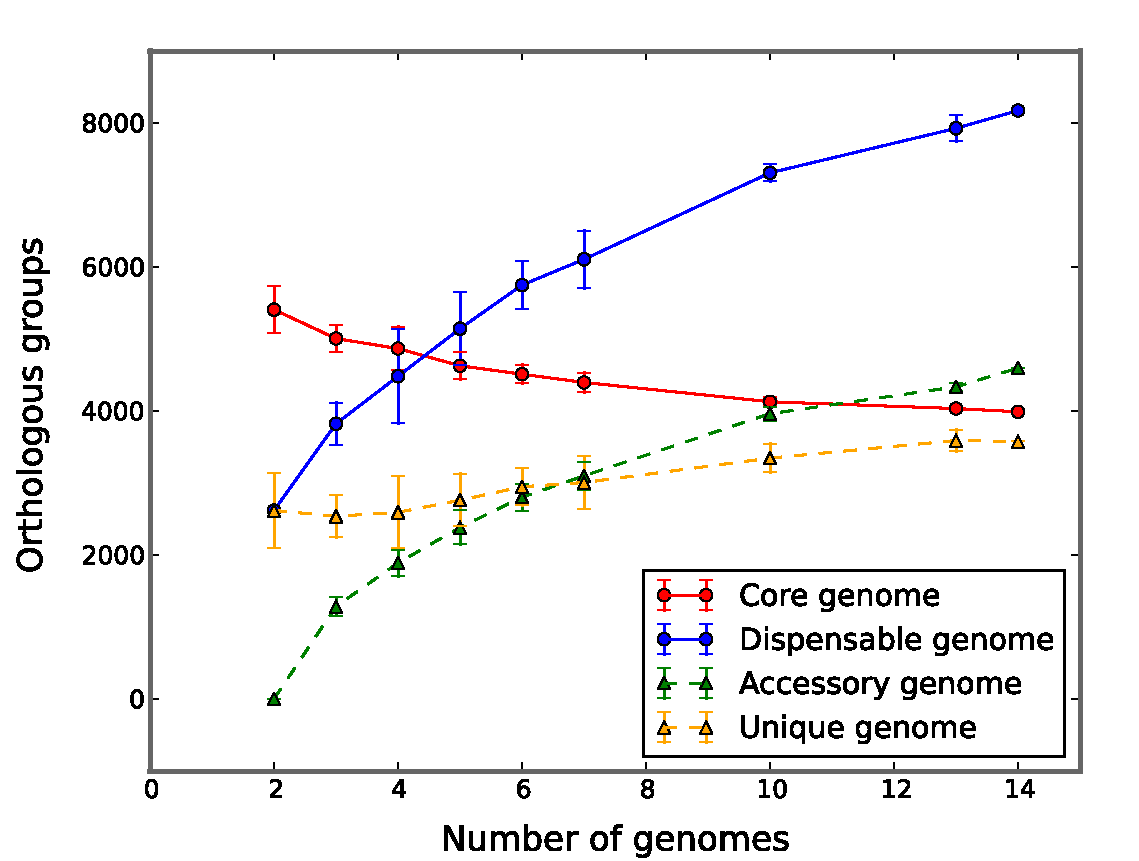
\includegraphics[width=0.8\textwidth]{figures/4/thesis_27}
	\caption{\label{fig:pangenome}\textbf{\textit{S. meliloti} pangenome permutations statistics.}\\Each point indicates the number of orthologs that are found in each pangenomic fraction. The trend lines on the median values are shown}
\end{figure}

The draft genome sequences of 10 \textit{S. meliloti} strains reported in Table \ref{tab:genomestats} were produced as described in Materials and Methods. The comparison of those 10 genomes with the complete sequences of the four strains already available at December 2011 (Rm1021, AK83, BL225C, SM11) showed that genome sizes varied from 6.69 Mbp (Rm1021) to 8.94 Mbp (5A14), with an average GC content of 61.9\%. The number of ORFs ranged from 6218 (Rm1021) to 8735 (5A14). The partial assembly of the new genomes was performed by contigs mapping with the four completely assembled genomes (Rm1021, AK83, BL225C, SM11): interestingly the newly sequenced genomes also possessed sequences belonging to the "rare" accessory plasmids such as pSINME01 and pSINME02 of strain AK83 and pSme11a and pSme11b of strain SM11. In particular all ten newly sequenced genomes contained sequences found in the accessory pSINME01 plasmid of strain AK83. Finally, 30\% of ORFs had no predicted function, while the proportion of proteins annotated by standard annotation sources ranged from 44.8\% (KEGG) to 83.3\% (Interpro). The highest annotation signal for all genomes was found, as expected, by homology with genes present in Rhizobase (86.4\%).
By comparing the 102082 ORFs found in the 14 genomes, a set of 12162/19003 orthologous groups (OGs) (using InParanoid or BBH respectively) was identified; a subset of 3989/4685 OGs was conserved across all genomes (core genome). The remaining 8173/14762 OGs were defined as members of the dispensable genome. Figure \ref{fig:pangenome} summarizes the results obtained comparing the 14 genomes of S. meliloti strains in relation to the core/dispensable genome and accessory and unique gene distribution. \textit{S. meliloti} appears to have an open pangenome, fitting the general Heaps law, $n = \kappa N\gamma$, with $\gamma$ higher than 0 \cite{tettelin2008comparative}, but has also a relatively stable core genome, accounting for slightly less than 4000 OGs. Genomic fluidity ($\phi$) is 0.32, in the range found for intra-specific polymorphism \cite{kislyuk2011genomic} and in agreement with that of other rhizobial species \cite{tian2012comparative}.

\begin{sidewaystable}[htbp]
  \tabcolsep 4pt
  \tiny
  \centering
    \begin{tabular}{rrcccccccccccccc@{}}
    \toprule
          &       & \multicolumn{14}{c}{\textbf{Strains}} \\
    \midrule
          &       & \textbf{1A42} & \textbf{5A14} & \textbf{A0641M} & \textbf{A0643DD} & \textbf{AE608H} & \textbf{AK11} & \textbf{AK75} & \textbf{C0431A} & \textbf{C0438LL} & \textbf{H1} & \textbf{Rm1021} & \textbf{AK83} & \textbf{BL225C} & \textbf{SM11} \\
    \multicolumn{1}{c}{\multirow{7}[1]{*}{\begin{sideways}\textbf{General stats}\end{sideways}}} & Length (Mb) & 7.16  & 8.94  & 7.95  & 7.35  & 7.35  & 6.84  & 6.99  & 7.09  & 7.06  & 6.92  & 6.69  & 7.14  & 6.98  & 7.5 \\
    \multicolumn{1}{c}{} & G+C content & 62.02 & 61.98 & 61.88 & 61.84 & 62    & 62.03 & 61.86 & 61.96 & 61.96 & 61.96 & 0.61  & 0.62  & 0.62  & 61.91 \\
    \multicolumn{1}{c}{} & Coding \% & 85.25 & 85.57 & 85.17 & 85.28 & 85.46 & 85.75 & 85.28 & 85.2  & 85.44 & 85.11 & 86.13 & 82.53 & 84.56 & 86.4 \\
    \multicolumn{1}{c}{} & Coding & 6106284 & 7652148 & 6774171 & 6269850 & 6279117 & 5868819 & 5963196 & 6037653 & 6035811 & 5892396 & 5763546 & 5893086 & 5901528 & 6479490 \\
    \multicolumn{1}{c}{} & ORFs  & 7374  & 8735  & 8411  & 7771  & 7197  & 6895  & 7555  & 7386  & 7242  & 6993  & 6218  & 6518  & 6359  & 7428 \\
    \multicolumn{1}{c}{} & rRNA  & 6     & 24    & 9     & 4     & 18    & 2     & 5     & 2     & 5     & 9     & 9     & 9     & 9     & 9 \\
    \multicolumn{1}{c}{} & tRNA  & 56    & 78    & 63    & 51    & 63    & 47    & 56    & 48    & 52    & 52    & 54    & 56    & 55    & 56 \\
    \multicolumn{1}{c}{\multirow{7}[0]{*}{\begin{sideways}\textbf{Annotation stats(\%) *}\end{sideways}}} & No function & 30.47 & 30.02 & 34.7  & 34.15 & 31.22 & 28.66 & 31.41 & 31.02 & 31.61 & 29.73 & 23.72 & 28.91 & 25.93 & 32.77 \\
    \multicolumn{1}{c}{} & ORFans & 3.38  & 3.57  & 3.67  & 3.35  & 1.92  & 3.16  & 3.45  & 2.4   & 3.02  & 2.89  & 1.74  & 2.75  & 0.3   & 0.7 \\
    \multicolumn{1}{c}{} & COG   & 69.53 & 69.98 & 65.3  & 65.85 & 68.78 & 71.34 & 68.59 & 68.98 & 68.39 & 70.27 & 76.28 & 71.09 & 74.07 & 67.23 \\
    \multicolumn{1}{c}{} & Interpro & 87.86 & 86.14 & 84.65 & 85.28 & 85.24 & 88.69 & 87.66 & 85.96 & 86.33 & 88.15 & 88.68 & 84.84 & 87.42 & 81.35 \\
    \multicolumn{1}{c}{} & GO    & 62.19 & 63.18 & 59.09 & 59.85 & 62.05 & 63.9  & 61.69 & 61.72 & 61.39 & 62.81 & 67.88 & 64.32 & 66.06 & 61.16 \\
    \multicolumn{1}{c}{} & KEGG  & 44.36 & 45.2  & 41.31 & 41.56 & 44.69 & 45.82 & 43.35 & 43.39 & 43.84 & 44.96 & 50.63 & 46.59 & 48.51 & 43.09 \\
    \multicolumn{1}{c}{} & Rhizobase** & 87.32 & 78.95 & 83.21 & 84    & 84.8  & 88.7  & 87.4  & 86.79 & 85.97 & 88.07 & 92.23 & 87.48 & 90.64 & 84.05 \\
    \multicolumn{1}{c}{\multirow{8}[0]{*}{\begin{sideways}\textbf{Replicon sizes (bp)}\end{sideways}}} & Chromosome & 3731100 & 4990772 & 4063405 & 3643054 & 3891677 & 3572765 & 3447294 & 3613238 & 3588400 & 3558302 & 3650000 & 3820000 & 3670000 & 3908022 \\
    \multicolumn{1}{c}{} & Chromid pSymB & 1588418 & 1878443 & 1754039 & 1593848 & 1630437 & 1565308 & 1647631 & 1558480 & 1626313 & 1603718 & 1680000 & 1680000 & 1690000 & 1632395 \\
    \multicolumn{1}{c}{} & Megaplasmid pSymA & 1396116 & 1506164 & 1457555 & 1307958 & 1285253 & 1387542 & 1518412 & 1389865 & 1313050 & 1374799 & 1350000 & 1310000 & 1610000 & 1633319 \\
    \multicolumn{1}{c}{} & pSINME01 & 209195 & 232672 & 111645 & 136588 & 125681 & 109990 & 76265 & 112338 & 94450 & 127226 &       & 260000 &       &  \\
    \multicolumn{1}{c}{} & pSINME02 &       &       &       & 11278 &       & 25905 &       &       & 7018  &       &       & 70000 &       &  \\
    \multicolumn{1}{c}{} & pSmeSM11b & 140640 & 178756 & 63273 & 122560 & 132879 & 11263 & 33722 &       & 71081 & 13413 &       &       &       & 181251 \\
    \multicolumn{1}{c}{} & pSmeSM11a & 14949 &       & 3811  & 232455 &       & 19702 &       & 14801 & 3810  &       &       &       &       & 144170 \\
    \multicolumn{1}{c}{} & Not mapped & 82306 & 155746 & 499985 & 304164 & 281255 & 151462 & 269272 & 398109 & 360652 & 245693 &       &       &       &  \\
    \bottomrule
    \end{tabular}%
  \caption{\textbf{Main features of the fourteen \textit{S. meliloti} genomes}\\
  			\textbf{*} \% on total ORFs\\
  			\textbf{**} Strain Rm1021 is excluded}
  \label{tab:genomestats}%
\end{sidewaystable}%

\subsubsection{Core and dispensable genome microevolution: replicon-based, intra-species differentiation}
\begin{figure}[!tb]
	\center
    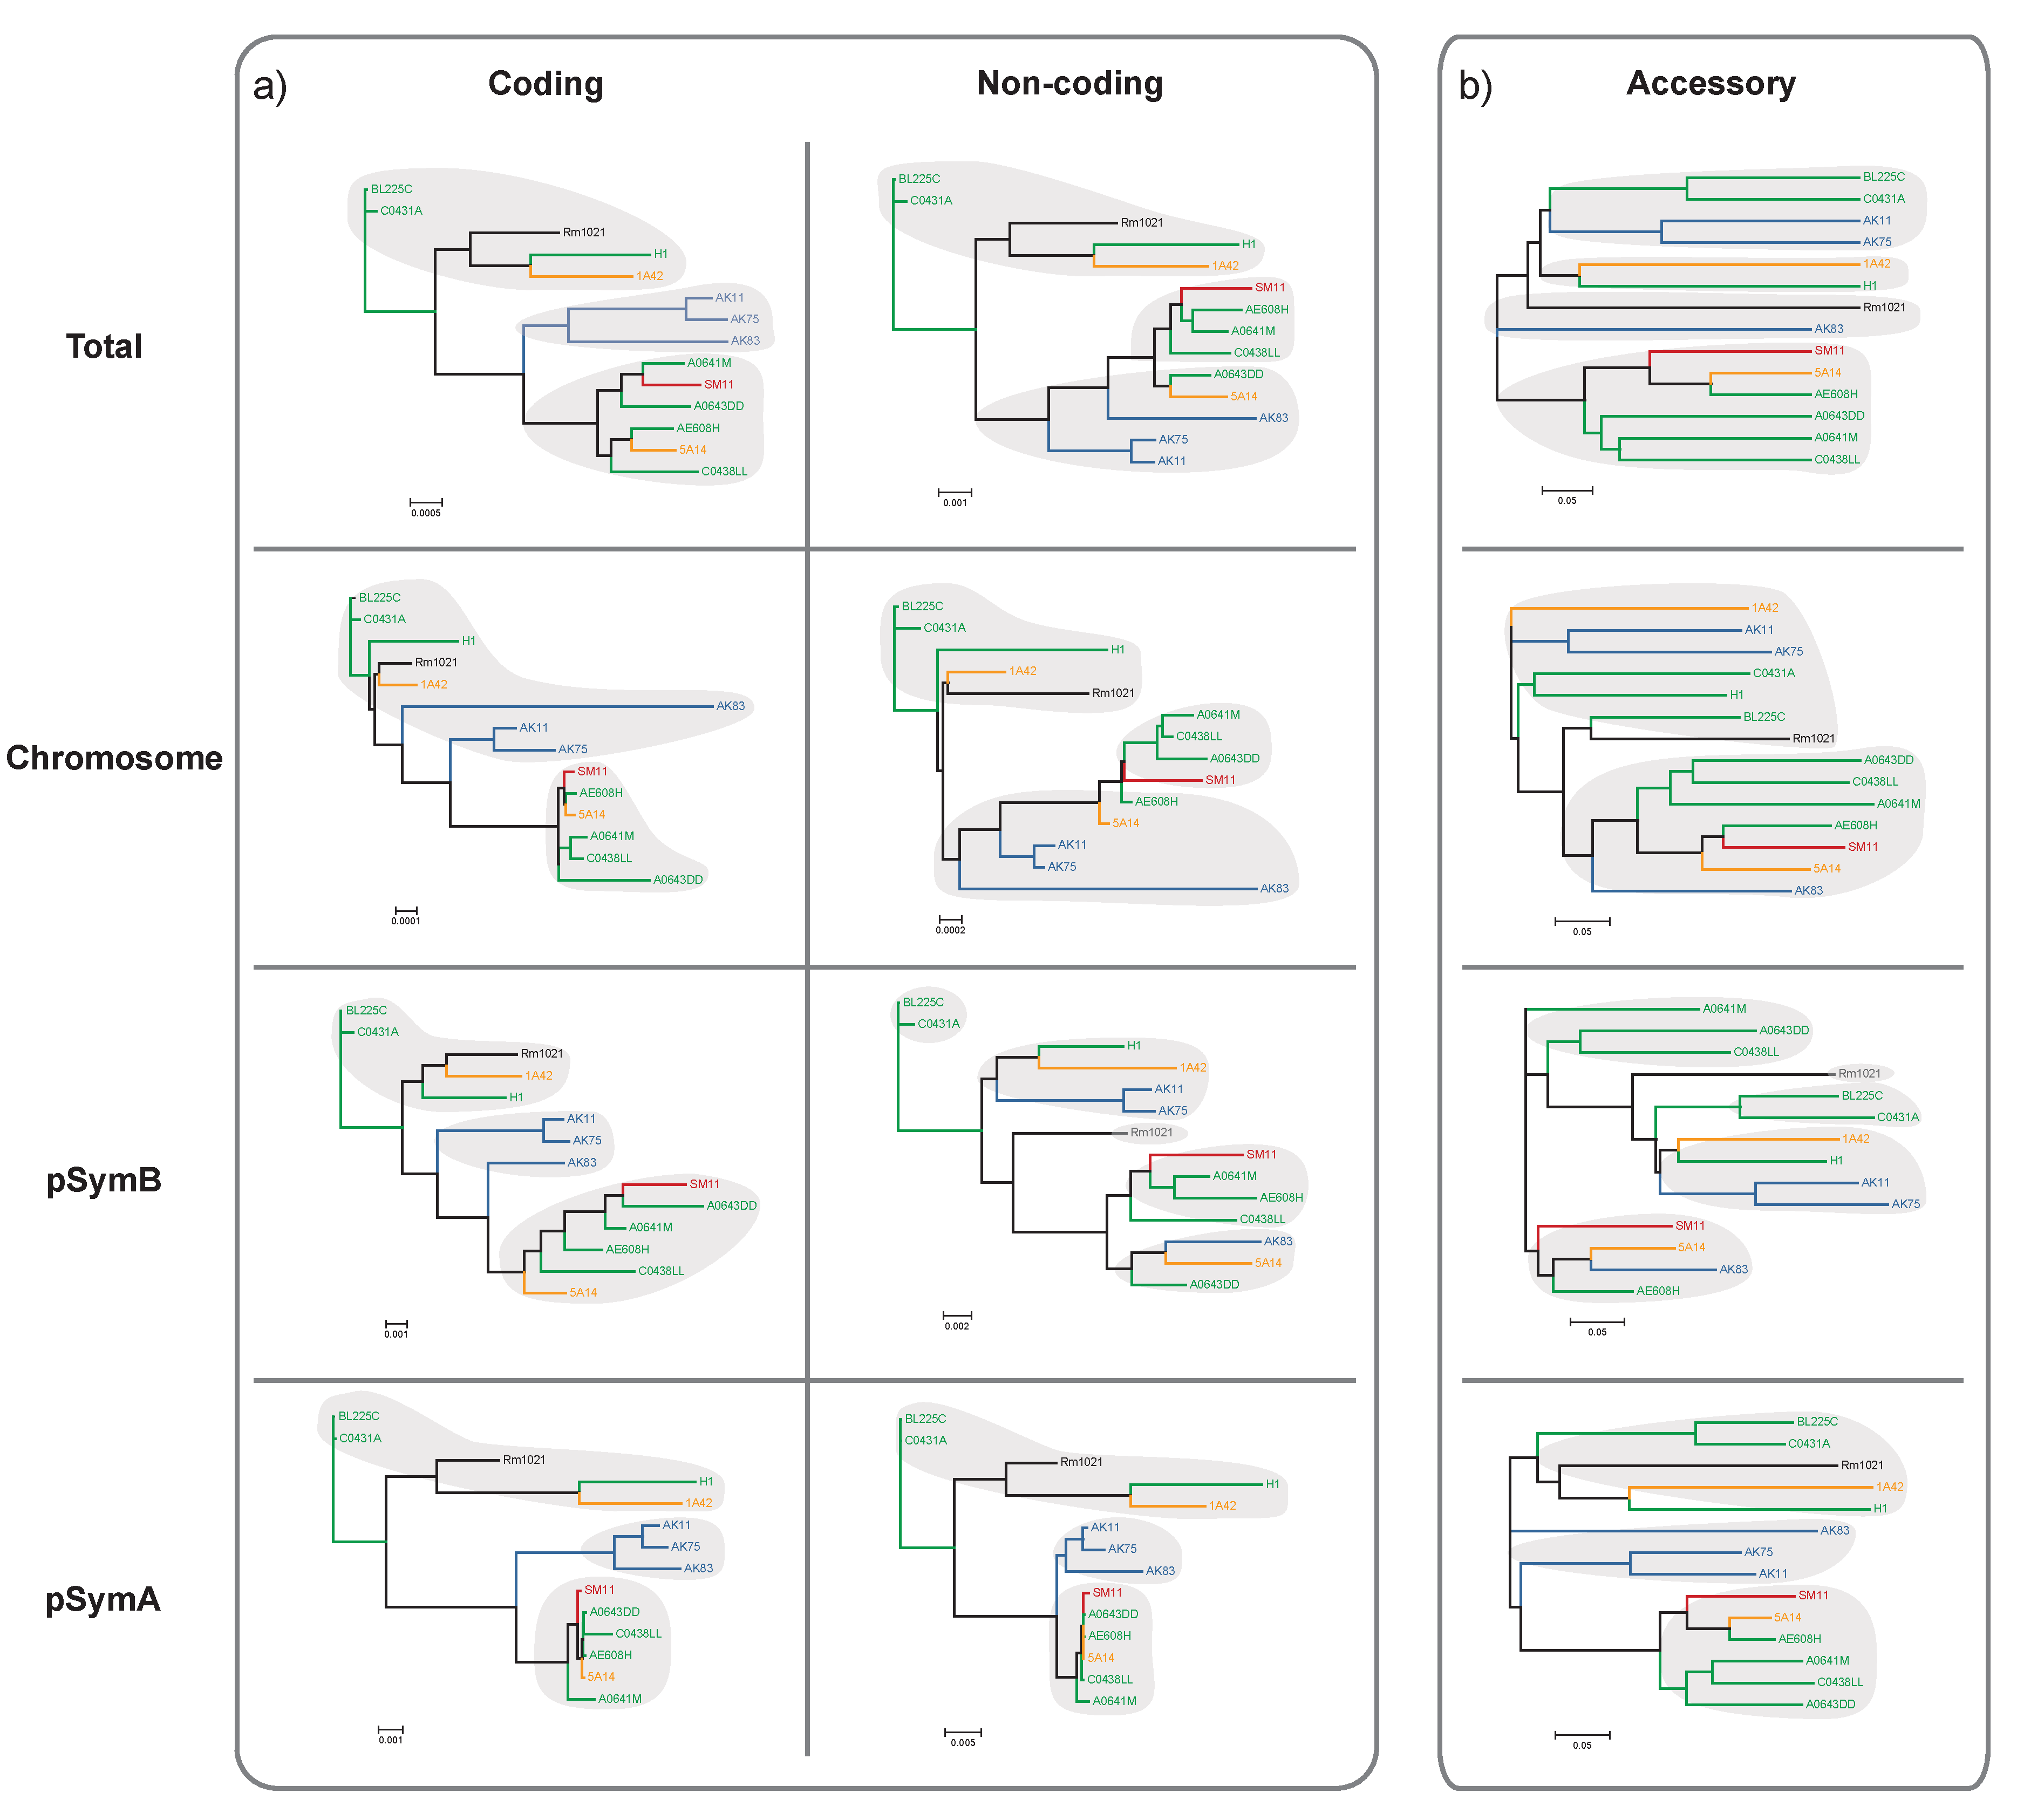
\includegraphics[width=1\textwidth]{figures/4/thesis_28}
	\caption{\label{fig:dendrogram}\textbf{Dendrograms of 14 the \textit{S. meliloti} strains based on pangenome content}\\Gray shades indicate the dendrogram’s clusters, strain names and branches are colored after the geographical origin of each strain (black: reference strain Rm1021; red: Germany; yellow: Iran; blue: Kazakhstan; green: Italy)\\
	a) Bayesian consensus dendrogram of \textit{S. meliloti} strains from core genome sequences alignments; both coding and non coding sequences dendrogram are reported\\
	b) Neighbor joining dendrograms with respect to the pattern of occurrence of 4602 accessory orthologs in the accessory genome.}
\end{figure}

Since the evolutionary dynamics in bacteria is different in the core and the dispensable genomes, we analyzed separately the genetic relationships among the 14 strains by using core genome loci and the pattern of differential occurrence of genes in the accessory genome. Moreover, for core genome, individual analyses of  the three main single replicons  and also of noncoding sequences were performed.
Concerning core genome diversity, four Bayesian dendrograms were reconstructed based on a concatenamer of nucleotide sequences of all core genome CDSs and noncoding sequences  mapped to the chromosome, pSymB and to pSymA (Figure \ref{fig:dendrogram}a). Moreover, a dendrogram with a concatenamer of nucleotide sequences of all CDS shared between the 14 S. meliloti strains, \textit{S. fredii} NGR234 and \textit{S. medicae} WSM419 was constructed, showing that S. meliloti strains, even though they are similar to \textit{S. fredii} NGR234 and \textit{S. medicae} WSM419, are well separated from these two different species. 
Additionally, to evaluate accessory genome relationships, a dendrogram from differential occurrence of accessory OGs was computed (Figure \ref{fig:dendrogram}b). In general from 2 to 5 clusters  were detected in the dendrograms of the 14 strains. The overall trees showed differential clusterizations: the coding fraction in the total tree and the coding fraction of chromid pSymB showed a 3-clusters arrangement that was also found in all the partitions of the megaplasmid pSymA; the megaplasmid shows then a similar signature, even at the accessory genome level. The Kazakhstan strains clustered  together in all the fraction of  pSymA and  in total and pSymB coding fraction in agrement with previous observations about the role of geographical isolation in \textit{S. meliloti} differentiation \cite{talebi2008diversity}. The chromosome showed a higher compactness, as expected for this more evolutionary conserved replicon, with 2 clusters for the coding and the accessory component, and 3 clusters for the non-coding component.The chromid pSymB showed the highest number of clusters, 3 for the coding component and 5 for the non-coding and the accessory components, suggesting a prominent role of this replicon for the differentiation within the \textit{S. meliloti} species.
To quantitatively evaluate the similarity between the accessory genome and core genome, Mantel's tests were carried out comparing the distance matrices obtained from core and accessory genome. Significant values for r Mantel's coefficient were found in all comparison, and the highest r value (r = 0.778) was obtained for pSymA, confirming earlier reports on the main role of pSymA on dispensable genome dynamics \cite{giuntini2005large}\cite{donini2009genome}. Moreover, distance matrices  of the three  main replicons CDSs were only partially (tough significantly) correlated  with r=0.623 (p<0.001) for pSymB-pSymA, r=0.510 for pSymA-chromosome and 0.524 (p<0.001) -for pSymB-chromosome. The same approach was used to compare trees of CDSs and surrounding noncoding regions, and, as expected, high correlation values were found r= 0.862, 0.902, 0.930 for chromosome, pSymB and pSymA, respectively, (p<0.001), suggesting a coevolution of CDS and of their noncoding flanking regions.  

\subsubsection{Evolutionary pressure on CDS: replicon-based patterns of positive selection}
\begin{figure}[!tb]
	\center
    \includegraphics[width=0.66\textwidth]{figures/4/thesis_29}
	\caption{\label{fig:positive}\textbf{Krona \cite{brian12interactive} pie chart of positively selected genes from 4685 BBH-retrieved ortholog groups}}
\end{figure}

To detect whether the different evolutionary forces acting on the three main replicons (chromosome, chromid pSymB, megaplasmid pSymA) effect gene evolution through purifying and positive selection, a genome-wide scanning for genes subjected to these evolutionary forces was performed following a general computational approach previously used in several bacterial species \cite{biswas2006genomic}\cite{petersen2007genes}. Within 2695 core aligned OGs, a total of 10 OGs under purifying selection were detected, as well as 313 positively selected OGs (Figure \ref{fig:positive}). The genes under purifying selection were evenly distributed in the three main replicons and comprised the fixO1 gene involved in nitrogen fixation, as well as bacA, which encodes for one of the key factors for the establishment of an effective symbiosis \cite{glazebrook1993rhizobium}, The highest percentage (11.4\%, 150 OGs) of genes under positive selection was found for OGs located (at least in one strain) on chromid pSymB, while 5.8\% (40 OGs) were located on megaplasmid pSymA and only 4.7\% of total aligned OGs (153) were located in the chromosome (Figure \ref{fig:positivereplicons}a). This high fraction of positively selected genes may match part of the phenotypic variability observed in natural populations \cite{biondi2009metabolic}. Notably, within the positively selected genes on pSymB, we detected genes coding for putative short chain oxidoreductases, which may have roles in hydroxybutyate accumulation \cite{jacob2008mutational}, or involved in osmotolerance, as eutA \cite{jebbar2005ectoine}, or in rhizopine uptake, as mocBD \cite{rossbach1994molecular}; interestingly, the mocD gene was found to exhibit also signs of purifying selection. On pSymA, we interestingly found positively selected genes involved in Nod Factor biosynthesis and host plant preference, such as nodCHLP \cite{roche1996common}, and the gene encoding for NoeB host specific nodulation protein, the FixB electron transfer flavoprotein alpha chain, involved in nitrogen fixation and, rpoE6/rpoE (RNA polymerase ECF sigma factor). For the chromosome, genes as ntrB (nitrogen regulation protein), xylA (xylose isomerase), flgF (flagellar basal-body rod protein), ureE (urease accessory protein) were found as positively selected, which may have a role in the adaptation to stress conditions \cite{bastiat2010dual}. We computed for each COG category the ratio between selected and not selected OGs (Figure \ref{fig:positivereplicons}b) in order to evaluate if several COG categories were more represented in the positively selected genes with respect to non-selected genes. Ten COG categories showed enrichment in positive selection: interestingly, within these 10 COGs, five COG related with environmental sensing and metabolic adaptation, namely K (Transcription), M (Cell envelope biogenesis, outer membrane), N (Cell motility and secretion), G (Carbohydrate transport and metabolism) and I (Lipid metabolism), showed the highest proportional differences (> 15\%). On the opposite, three COGs, one of which containing mainly housekeeping functions (J, Translation, ribosomal structure and biogenesis; O, Post translational modification, protein turnover, chaperones and F, Nucleotide transport and metabolism), showed the lowest proportional differences (< -25\%) with the non-selected genes. It should be mentioned that indeed the chromid pSymB is particularly rich in carbohydrate transporters \cite{finan2001complete} and was supposed to play important roles in the survival of the bacterium under highly variable nutritional conditions encountered in the soil and rhizosphere. Under this view it not unexpected that an higher number of positively selected genes are resident on this replicons, suggesting that the chromid pSymB is a hot spot for adaptation in free living (non-host) highly diverse conditions, which indeed challenge bacterium’s fitness. Up to now, most of genome-wide searches for positively selected genes have been performed on pathogenic species (see for instance \cite{petersen2007genes}). These studies showed that surface proteins encoding genes are among the most relevant categories of positively selected genes, suggesting a strong role of host immune system in strain diversification. By paralleling these data, we could suppose that the evolutionary role played by host immune system variability for pathogenic bacteria is played by environmental carbohydrate scavenging by soil and rhizosphere bacteria. However, statistical evidences of positive selection should be considered with caution, since different methods may yield very different results. In a recent paper on a panel of \textit{S. meliloti} and \textit{S. medicae} strains \cite{epstein2012population}, the use of a different metrics (DTH test \cite{zeng2006statistical}) indicated that also some non essential symbiotic functions may be under positive selection, tough curiously no overlap of positively selected orthologs was found for the two species.

\begin{figure}[!t]
	\center
    \includegraphics[width=0.66\textwidth]{figures/4/thesis_30}
	\caption{\label{fig:positivereplicons}\textbf{Detection of positively selected sites in the three main \textit{S. meliloti} replicons}\\
	a) The proportion of positively selected sites detected with respect to the total number of genes present is reported. Asterisks indicate significant enrichment (P<0.003, 3 standard deviations) of positively selected genes\\
	b) Difference between relative proportions of each COG category between selected and non selected core genes. All differences except B are significant}
\end{figure}

\subsubsection{Taxonomic distribution: chromid genes are widespread in distant taxa}
\begin{figure}[!t]
	\center
    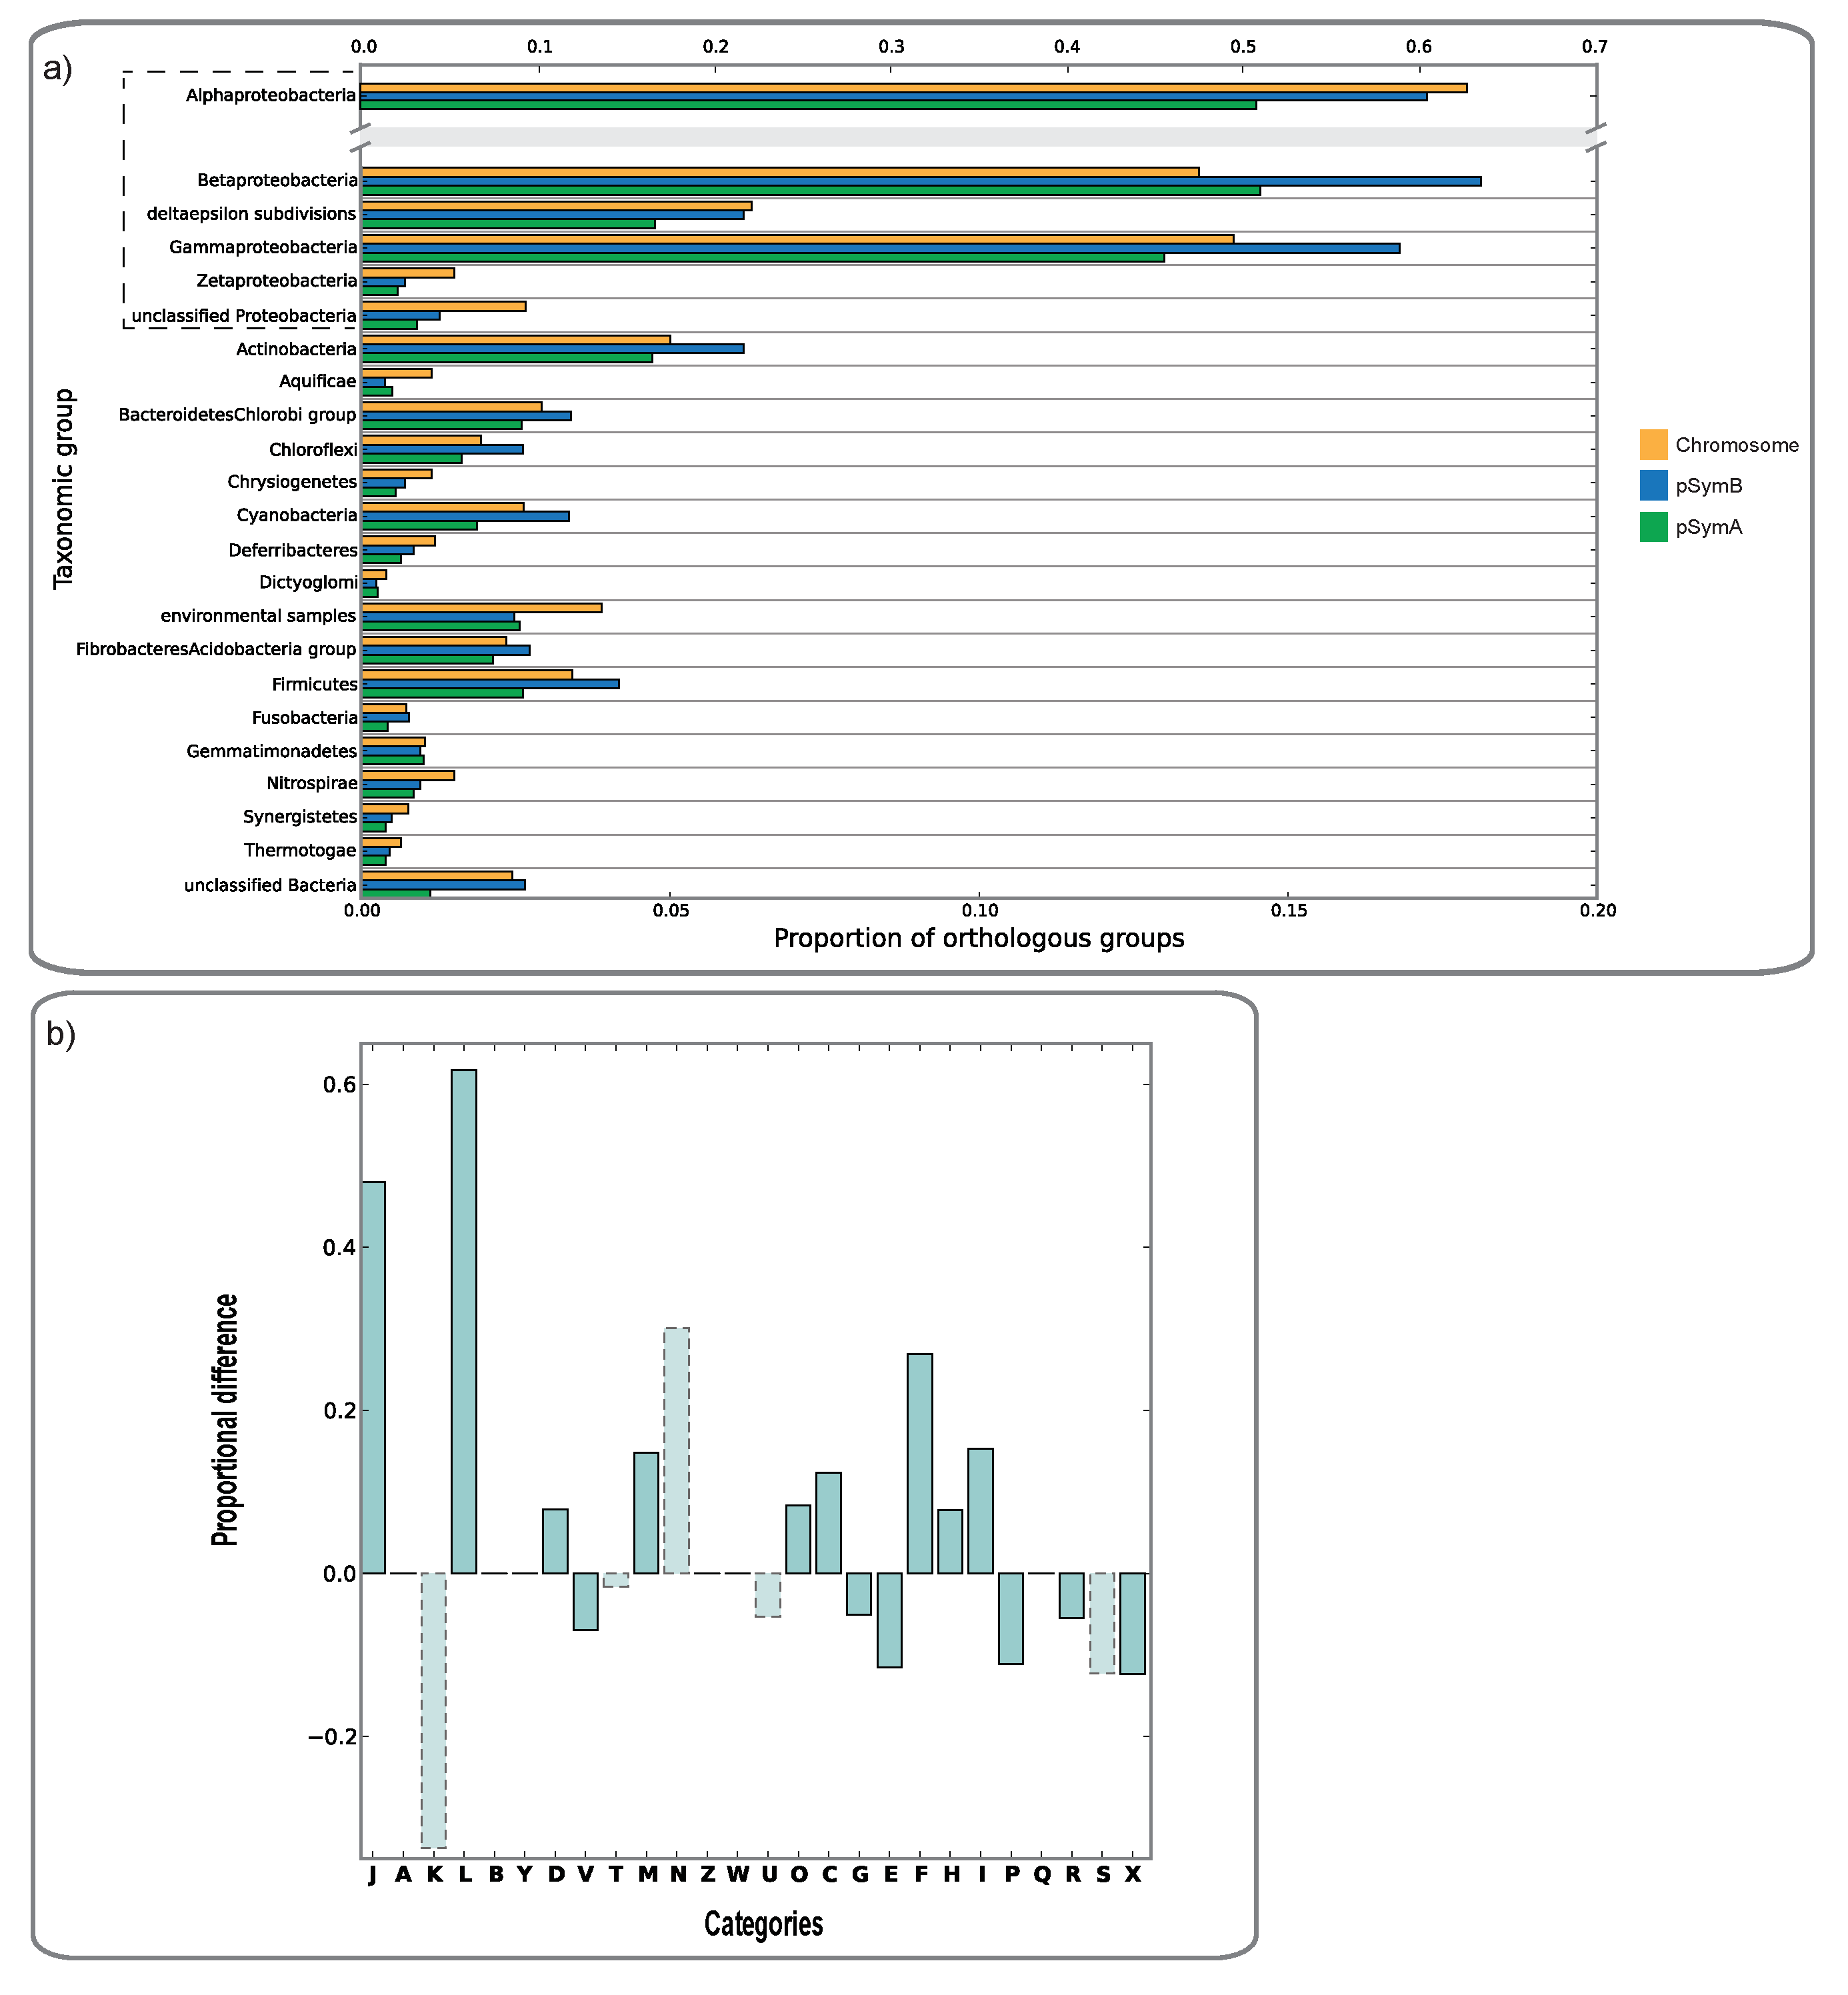
\includegraphics[width=0.9\textwidth]{figures/4/thesis_31}
	\caption{\label{fig:taxa}\textbf{Taxonomic distribution of the \textit{S. meliloti} pangenome}\\
	a) Taxonomic distribution of the OGs mapped to each replicon: for each taxonomic group, the proportion of the orthologs for each replicon having a significant hit is reported\\
	b) Difference between relative proportions of each COG category between proteobacterial hits and non-proteobacterial hits. Solid histograms mark categories with significant differences}
\end{figure}

To infer the phylogenetic origin of dispensable genome and its potential differences with respect to the phylogenetic relationships of the core genome, a homology analysis on taxonomic partitions of the nr database \cite{pini2011plant} was carried out in order to define the bacterial (and proteobacterial) phylogenetic groups to which each replicon shows the highest similarity (Figure \ref{fig:taxa}). When analyzing the orthologs with respect to their position on the three main replicons (Chromosome, pSymB and pSymA, Figure \ref{fig:taxa}a), several bacterial classes, notably \textit{Betaproteobacteria} and \textit{Gammaproteobacteria} had the highest number of matches for orthologs harbored by pSymB, while orthologs located on the chromosome and on pSymA had a (similar) lower proportion. This evidence may suggest a wider scenario for chromids evolution, which may have originated by (very ancient) gene transfer events by distant relatives and then contributed in the emergence of new taxa (e.g. genera) \cite{harrison2010introducing}. However, analyses on a large-scale dataset are needed to evaluate the taxonomic distribution of chromid-harbored genes in several genera. 
Finally, to provide functional insights over the orthologs that \textit{S. meliloti} shares with proteobacterial and non-proteobacterial taxa, the differences between hits on non-proteobacterial and proteobacterial taxa were computed for each COG category. Results of the analysis are shown in Figure \ref{fig:taxa}b. Interestingly, positive values of proportional differences were obtained for several COGs involved in housekeeping functions (as J, L, D, M, O, C, F, H, I), indicating that orthologs for these functions are significantly shared with also non-proteobacterial taxa. Conversely, COGs coding for "accessory" functions, as defense mechanisms (V), carbohydrate and aminoacid metabolism (G and E), secondary metabolites (P) are more represented in hits on proteobacterial taxa than in non-proteobacterial taxa.

\subsubsection{Structural evolution through rearrangements on a shared backbone}
\begin{figure}[!t]
	\center
    \includegraphics[width=1\textwidth]{figures/4/thesis_32}
	\caption{\label{fig:structure}\textbf{Structural alignments of the 14 \textit{S. meliloti} genomes}\\
	Alignment between genomes are reported, following the order of the overall Bayesian dendrogram (Figure \ref{fig:dendrogram}), the presence of core, accessory and unique contiguous regions of orthologs whose length is over 10 kbp is reported}
\end{figure}

To infer potential structural features (uneven or even distribution along the replicons) of the dispensable genome in the 14 strains, the 10 draft genomes were assembled using CONTIGuator \cite{galardini2011contiguator}, and the resulted reconstructed putative replicons were aligned (see Materials and  methods) to the complete genomes of AK83, BL225C, Rm1021 and SM11 strains (Figure \ref{fig:structure}). Interestingly, the dendrogram of genetic relationships between strains was well mirrored by structural features of the same strains. It is worth notice that, in fact, the three main clusters present in the dendrogram (containing Rm1021, SM11 and AK83, respectively), correspond to the presence of large inversions. Another interesting feature is the evidence that the dispensable genome and especially unique genes fractions are mainly distributed in clusters (blue and green zones, respectively). In particular pSymA contained, as expected, a higher proportion of accessory and unique contiguous blocks, while pSymB and the chromosome contained a higher proportion of core contiguous blocks, in agreement with earlier reports \cite{giuntini2005large}\cite{galardini2011exploring}. Particularly interesting is also the abundance of unique gene clusters in pSymA (roughly 10\% of the total, against the 5\% proportion of the chromosome and the chromid), compared to the other large replicons (Figure \ref{fig:structure2}); in the two smaller plasmids a significant higher fraction of dispensable contiguous block is present, as expected  in such small accessory plasmids.
\begin{figure}[!tb]
	\center
    \includegraphics[width=0.77\textwidth]{figures/4/thesis_33}
	\caption{\label{fig:structure2}\textbf{Structural analysis of the 14 \textit{S. meliloti} genomes}\\
	Proportion of contiguous regions for each pangenomic category in each replicon}
\end{figure}
The arrangement of the unique gene fraction in blocks on \textit{S. meliloti} genomes is particularly relevant, since unique genes are used as models for inferring de novo gene evolution. Unique gene evolution models hypothesize that transcriptional and translational events in noncoding regions or sporadic phage integrations are fixed and, after passing the natural selection filter, lead to the emergence of unique (novel) genes \cite{yomtovian2010composition}\cite{carvunis2012proto}. In this perspective, the slightly higher abundance of unique and dispensable genes found on pSymA makes sense with either a higher proportion of mobile genetic elements there residents \cite{biondi2011spread} and with the lower percentage of protein-coding DNA (and consequently higher intergenic regions length) in pSymA, with respect to the chromosome and to pSymB \cite{galardini2011exploring}.
\begin{figure}[!tb]
	\center
    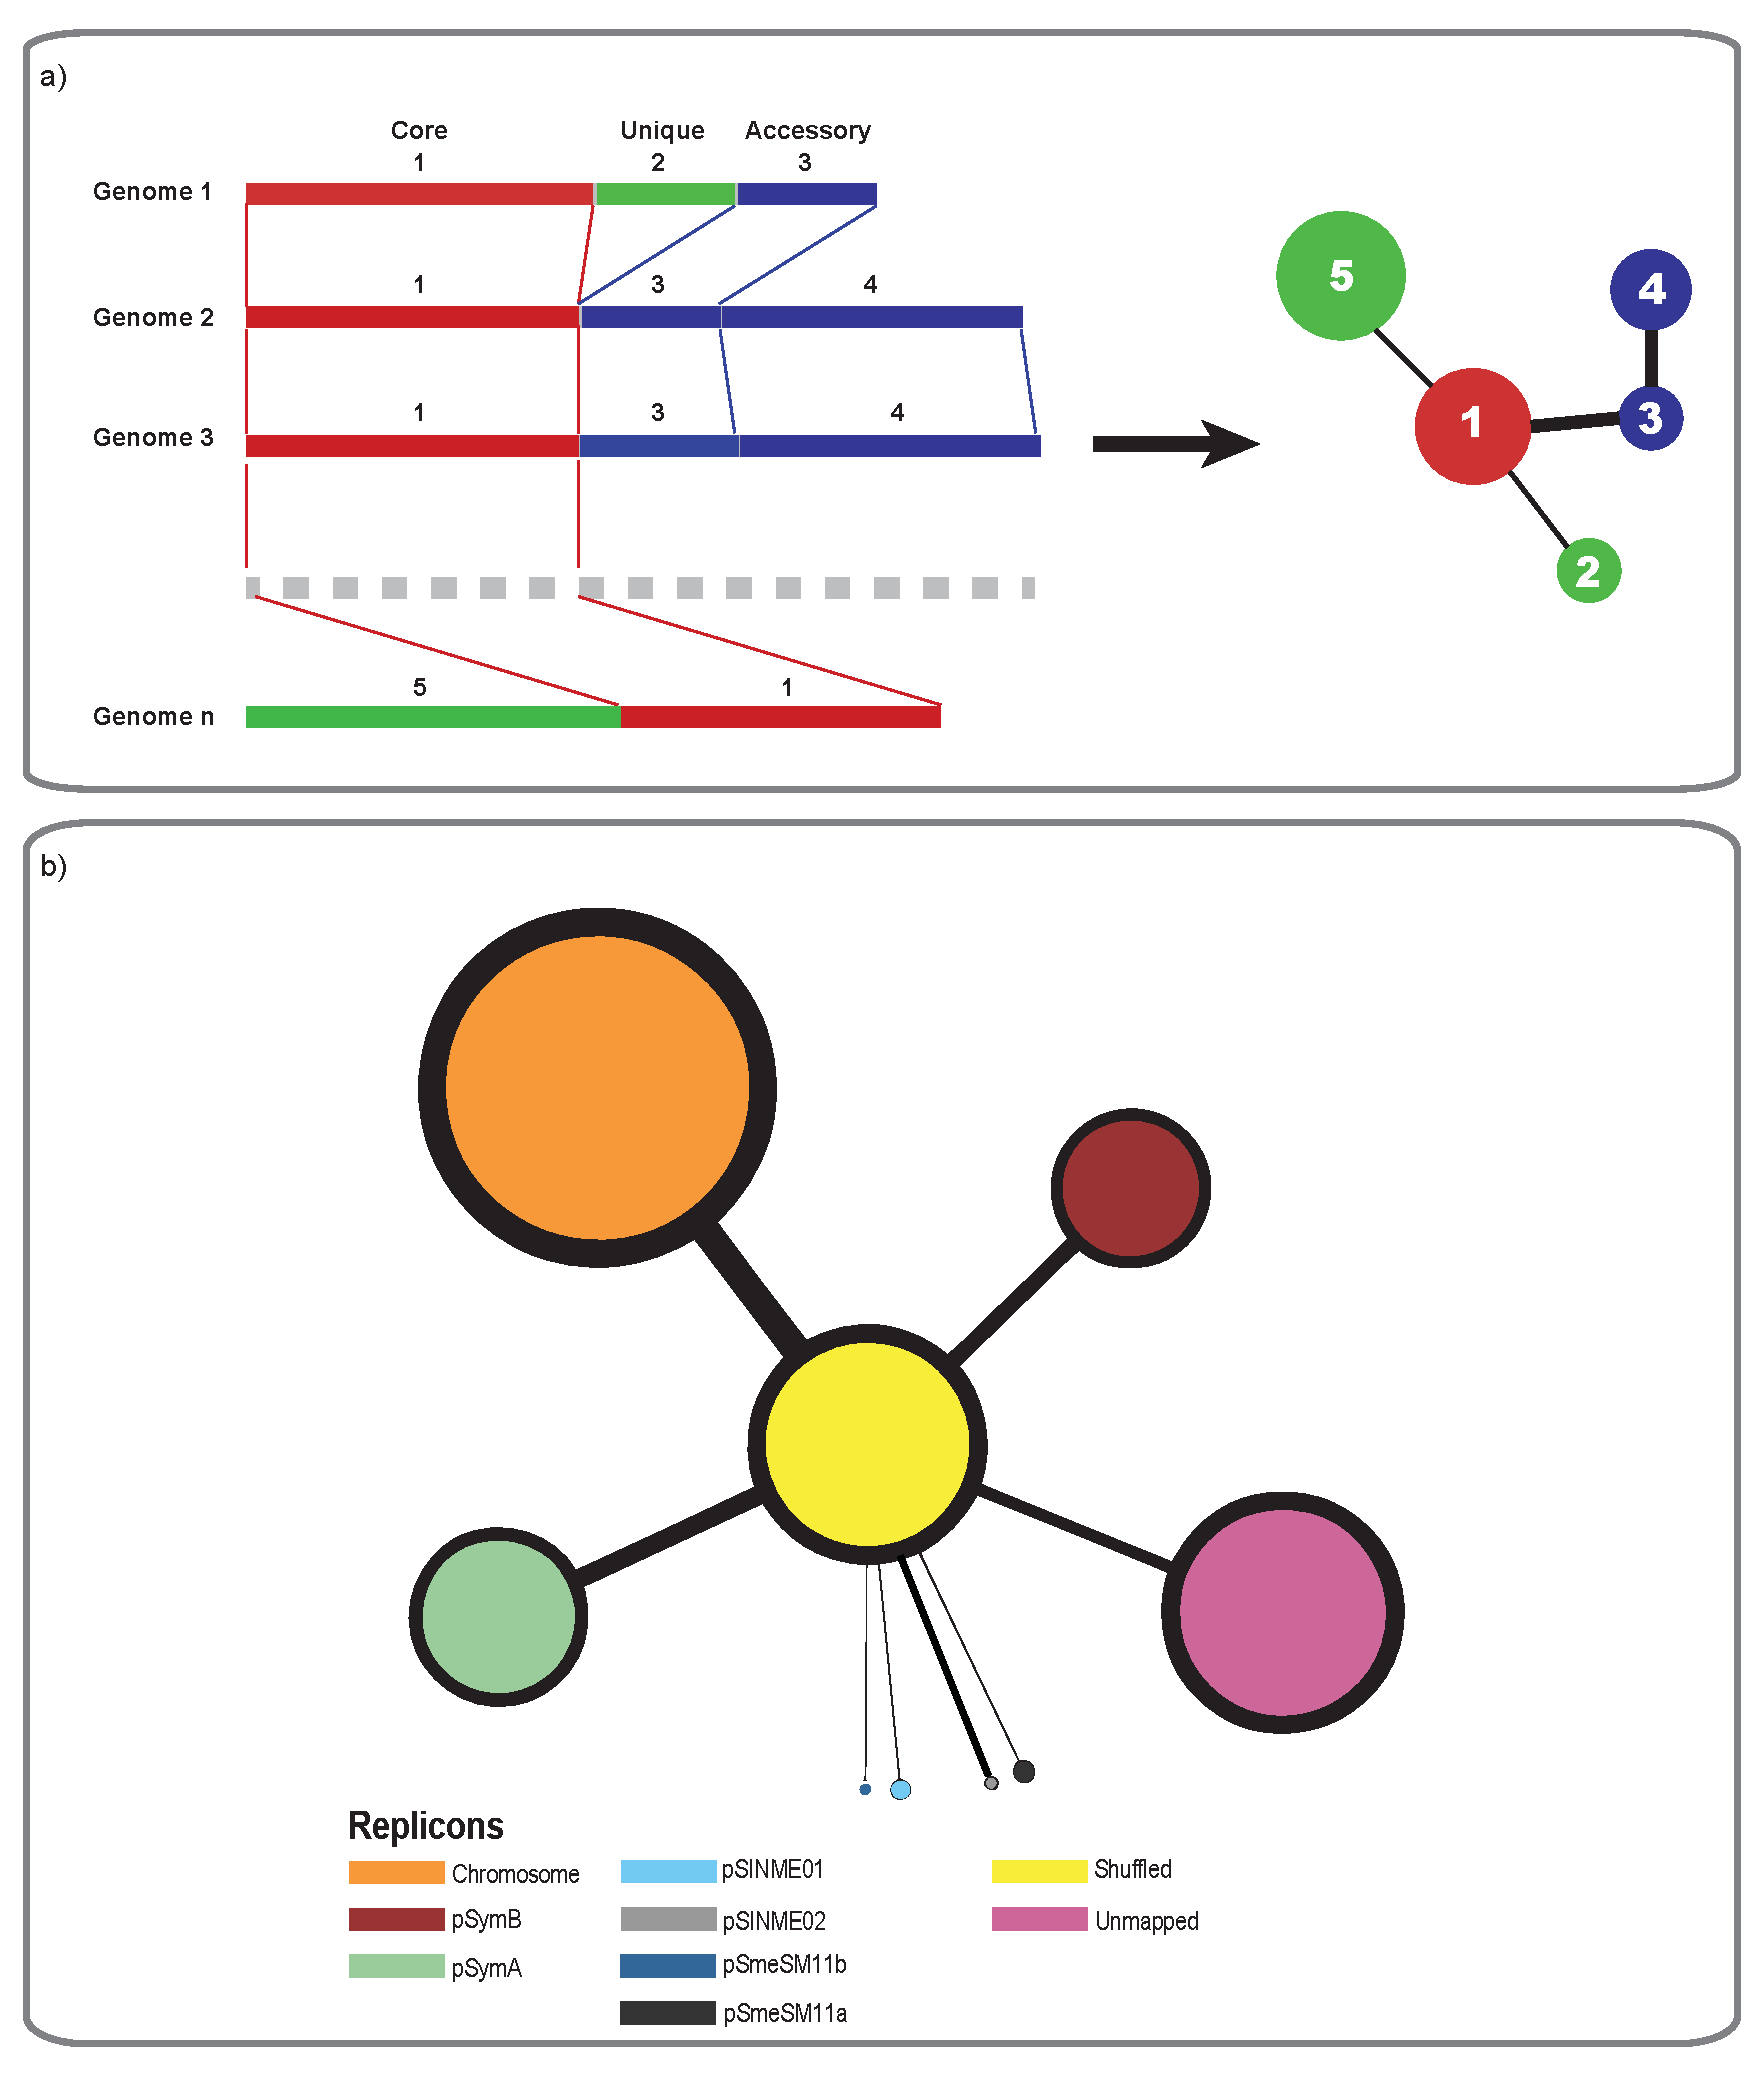
\includegraphics[width=0.77\textwidth]{figures/4/thesis_34}
	\caption{\label{fig:network}\textbf{Proximity network construction and statistics}\\
	a) Explanatory proximity network construction details\\
	b) Block model simplified version of the proximity network, obtained dividing the nodes according to their replicon of origin; nodes and edges sizes are proportional to the number of orthologs and number of links observed, respectively}
\end{figure}
To understand how the genomic structure evolves, a deeper structural analysis was then performed through the exploitation of the DNA proximity network; the network has been constructed so that each node represents a nucleotide region present in one or more genomes, while the edges represent the proximity of each region to the others on one or more genomes, the weight of the edge being proportional to the number of times each link is observed in the whole pangenome (Figure \ref{fig:network}a). A total number of 24518 nodes (with an average size of 894 bp) and 36781 edges were added to the network: each node was assigned to its replicon of origin, “Shuffled” (if the node was mapped to more than one replicon in the pangenome) or “UnMapped” (if the node wasn’t assigned to any replicon). A simpler block-model network was then constructed using the replicon information, the nodes size proportional to the bases mapped and the edges proportional to the number of links between each replicon (Figure \ref{fig:network}b): as expected the largest node is that representing the chromosome, with 6.58 Mb mapped in the whole pangenome, followed by the Shuffled and UnMapped nodes (4.34 and 4.38 Mb respectively); interestingly, the megaplasmid pSymA showed a higher number of bases than the chromid (3.19 and 2.83 Mb respectively), a feature that can be explained by the higher number of accessory regions mapping to this replicon, which in fact leads to a megaplasmid which is larger than the chromid in pangenomic terms.

\begin{sidewaystable}[htbp]
  \centering
  \tiny
    \begin{tabular}{rrrrrrrrrrr}
    \toprule
          & \multicolumn{10}{c}{\textbf{DNA Proximity Network cluster}} \\
    \midrule
          & \multicolumn{1}{c}{All} & \multicolumn{1}{c}{Mapped} & \multicolumn{1}{c}{Shuffled} & \multicolumn{1}{c}{Chromosome} & \multicolumn{1}{c}{pSymB} & \multicolumn{1}{c}{pSymA} & \multicolumn{1}{c}{pSINME01} & \multicolumn{1}{c}{pSmeSM11b} & \multicolumn{1}{c}{pSINME02} & \multicolumn{1}{c}{pSmeSM11a} \\
    \textbf{Average Degree*} & 3.00  & 2.91  & 2.63  & 2.98  & 2.88  & 2.77  & 2.43  & 2.79  & N/A   & 2.42 \\
    \textbf{Std-dev Degree*} & 1.00  & 0.97  & 0.81  & 1.00  & 0.97  & 0.89  & 0.73  & 0.89  & 0.00  & 0.72 \\
    \textbf{Replicon Assortativity} & 0.67  & 1.00  & N/A & N/A & N/A & N/A & N/A & N/A & N/A & N/A \\
    \textbf{Major component Weighted size} & 1.00  & 0.21  & 0.19  & 0.43  & 0.17  & 0.29  & 0.13  & 0.56  & 0.04  & 0.13 \\
    \textbf{Boundary weighted size**} & N/A & 0.34  & N/A & 0.27  & 0.34  & 0.44  & 0.94  & 0.68  & 1.00  & 0.70 \\
    \bottomrule
    \end{tabular}%
  \caption{\textbf{DNA proximity network statistics}\\
  \textbf{*} Considering nodes with degree > 1\\
  \textbf{**} Nodes having at least a link to the shuffled cluster}
  \label{tab:proximity}%
\end{sidewaystable}%

A series of network statistics were computed for the overall network (“All”), the nucleotidic regions univocally mapped to one replicon (“Mapped”), the shuffled regions (“Shuffled”) and the single replicons (Table \ref{tab:proximity}): the overall network had the highest average node degree (\textasciitilde 3), meaning that each node is connected to three other nodes on average, resulting in a relatively non-conserved structure in the whole pangenome; when considering the replicon assortativity (a measure of how much each node tends to be closer to a node coming from the same replicon), the highest value is found for the “Mapped” component, meaning that when the shuffled nodes are removed from the proximity network, the single replicons have no links connecting each other, thus suggesting indeed the presence of a conserved core structure for each replicon. This finding was further confirmed looking at the size of the major connected component (that is, the largest subgraph in which each node can be reached from any other node): only \textasciitilde 21\% of the “Mapped” component was linked in a single cluster; when considering the larger replicons, the chromosome was found to have the larger fraction of its content present in a single cluster (\textasciitilde 43\%), while lower values for the other two replicons, meaning that the chromosome structure is evolutionary more conserved, with nearly half of its nucleotidic content with a conserved structure. As expected, the opposite trend was observed when looking at the fraction of genes of each cluster that were present in the “boundary” to the shuffled component (which are the nodes having an edge to a node in the shuffled component), ranging from \textasciitilde 27\% (chromosome) to 100\% (pSINME02), with the megaplasmid having the highest proportion of nodes in boundary among the larger replicons (\textasciitilde 44\%), meaning that the megaplasmid experienced a higher number of rearrangements than the other replicons. This observation is confirmed when looking at the number of putative transposases encoded in each replicon, with the megaplasmid pSymA harboring almost three times the transposases found in the chromosome and in the chromid, a feature that could explain the higher fluidity of this replicon.
\begin{table}[htbp]
  \centering
    \begin{tabular}{rrrrr}
    \toprule
          & \textbf{All} & \textbf{Chromosome} & \textbf{pSymB} & \textbf{pSymA} \\
    \midrule
    \textbf{Number of chains} & 1035  & 349   & 118   & 60 \\
    \textbf{Total length (Mb)} & 2.68  & 2.03  & 0.51  & 0.27 \\
    \textbf{Length proportion*} & N/A   & 0.54  & 0.31  & 0.18 \\
    \textbf{Average length (bp)} & 5391.9 & 5819.7 & 4342.4 & 4502.2 \\
    \textbf{Std-size size (bp)} & 6561.6 & 6281.8 & 6257.8 & 5522.5 \\
    \textbf{Average degree**} & 2.00  & 2.00  & 2.00  & 2.00 \\
    \textbf{Std-dev degree**} & 0.00  & 0.00  & 0.00  & 0.00 \\
    \bottomrule
    \end{tabular}%
    \caption{\textbf{DNA backbones statistics}\\
    			\textbf{*} Replicon size is the average replicon length in the four complete \textit{S. meliloti} genomes\\
			\textbf{**} Considering nodes with degree > 1}
	\label{tab:chains}%
\end{table}%
To inspect if there was a conserved structural backbone in the pangenome, the overall network was divided using a filter on the links weight, that are proportional to the number of times two nucleotide regions are seen as adjacent in the whole pangenome (Figure \ref{fig:network}a), leading to the definition of “DNA backbones”, which are the largest conserved genomic structures in the \textit{S. meliloti} pangenome; both the overall backbones and the replicon specific backbones were computed (Table \ref{tab:chains}).  For all the three categories used, only linear backbones were found (degree=2), with a similar average length of roughly 5'000 bp, meaning that the underlying mechanisms of formation and evolution of these backbones may be similar in the three replicons; on the other hand, the proportion of replicons conserved in a backbone varies between each replicon: roughly half of the chromosome is conserved and contained in a single backbone, one third of the chromid pSymB is conserved, while just 18\% of the megaplasmid pSymA is conserved; thus, even though the mechanisms of structural evolution are similar in each replicon, the extent of the structural variability is different.

\subsubsection{An evolutionary scenario for multipartite bacterial genomes}
\begin{figure}[!tb]
	\center
    \includegraphics[width=0.6\textwidth]{figures/4/thesis_35}
	\caption{\label{fig:replicons}\textbf{Tasks and evolutionary differences of replicons in \textit{S. meliloti}}\\
	Pie charts indicate the proportion of each replicon that is present in the DNA backbones. The arrows indicate the transmission mechanism: vertical inheritance (two arrows) or HGT (radial arrows)}
\end{figure}

Bacterial genomes are classically described by the “\textit{E. coli} rules”, in which the genome is composed by one chromosome, plus additional plasmids which often carry non-essential functions \cite{krawiec1990organization}. However, this approximation fails to describe several bacterial species, for which large additional replicons are present as secondary chromosomes, megaplasmids, etc. Recently, the term “chromid” has been proposed \cite{harrison2010introducing} to describe large replicons which contain plasmid-type replication systems but also essential genes for growth and survival. 
Here the analysis of 14 \textit{S. meliloti} multipartite genomes allowed us to show that each replicon behave as partially independent evolutionary unit, suggesting that the multi-replicon structure in some bacterial species may be functional to the physical separation of different functions but also of different evolutionary pressures. This is the case of \textit{S. meliloti} which exploits multiple ecological niches (soil, rhizosphere, root nodule, plant endosphere etc. \cite{pini2012exploring}), In particular the chromid pSymB behave as an independent evolutionary unit, and our data suggest that the biological and evolutionary meaning of chromids is larger than previously hypothesized, playing a considerable role at the intraspecific level, in addition to genera differentiation \cite{harrison2010introducing}. Indeed chromids could also have a role in species differentiation as genomic elements for adaptation through individual genes evolution, while the plasmids and megaplasmids are more prone to structural evolution (e.g. via horizontal gene transfer). 
The overall evolutionary scenario of the three main S. meliloti replicons could be approximated as in Figure \ref{fig:replicons}. The chromosome contains most of the housekeeping functions and originated mainly by vertical descent from \textit{S. meliloti} phylogenetic relatives. The chromid pSymB indeed is mainly vertically transmitted in the genus Sinorhizobium \cite{harrison2010introducing} \cite{bailly2011population}, but it also acquired genes from distant relatives by primordial horizontal gene transfer events. Functions of pSymB are mainly related to exploitation of environment and evolution takes place through positive selection of genes involved in environmental exploitation. Finally, the megaplasmid pSymA, as alien element (its GC content is significantly different from those of chromosome and of chromid \cite{galibert2001composite}) is the replicon devoted to the introduction of genomic novelties (as new genes coming by horizontal gene transfer). It is worth to remember that the most relevant bioprocess of rhizobia (symbiotic nitrogen fixation) is indeed linked to this last replicons, and that functional diversification via purifying selection seems to act also on a number of symbiotic-related genes; moreover, unlike the other replicons, both core and accessory fractions show a similar pattern, indicating similar evolutionary patterns for the conserved and variable fractions in this replicon. Interestingly, at the structural level, the network analysis highlighted the presence of stable core structures in each replicons, the chromosome having the largest conserved network, followed by the pSymB chromid and finally by the pSymA megaplasmid, which was confirmed as a hot spot for structural rearrangements.
In conclusion this study demonstrates that the evolution of the \textit{S. meliloti} pangenome shows two opposite behaviors: a strongly conserved genome that evolves by positive selection on genes related to survival in complex environments, and an highly variable fraction that most likely contributes to structural fluidity and the emerging of new functions. The conserved genome signature is replicon-specific, while for the variable part the signature is more strain-specific. It is not clear yet if this model is applicable to other multipartite bacterial genomes, which contains both chromids and plasmids and may have different ecological features (e.g. Brucella, Variovorax, Vibrio, etc. for a list of genera see \cite{harrison2010introducing}). However future population genomics analyses on other species with these features will help elucidating the evolutionary role of multipartite genomes in bacteria.


%%-----------
%% Backmatter
%%-----------
\backmatter
\chaptermark{Bibliography}
\renewcommand{\sectionmark}[1]{\markright{#1}}
\bibliographystyle{unsrt}                           %Use alpha codes for references
\sectionmark{Bibliography}
\addcontentsline{toc}{chapter}{Bibliography}        %Force addition of Bibliography to TOC    
\bibliography{References}